%% LyX 2.2.3 created this file.  For more info, see http://www.lyx.org/.
%% Do not edit unless you really know what you are doing.
\documentclass[11pt,english]{article}
\usepackage{mathpazo}
\usepackage{avant}
\usepackage{courier}
\usepackage[T1]{fontenc}
\usepackage[latin9]{inputenc}
\usepackage[letterpaper]{geometry}
\geometry{verbose,tmargin=1in,bmargin=1in,lmargin=1in,rmargin=1in,headheight=0in,headsep=0in}
\usepackage{color}
\usepackage{babel}
\usepackage{array}
\PassOptionsToPackage{normalem}{ulem}
\usepackage{ulem}
\usepackage{listings}
\usepackage{color}
\usepackage[unicode=true]
 {hyperref}
\usepackage{graphicx}

\makeatletter

%%%%%%%%%%%%%%%%%%%%%%%%%%%%%% LyX specific LaTeX commands.
%% Because html converters don't know tabularnewline
\providecommand{\tabularnewline}{\\}

%%%%%%%%%%%%%%%%%%%%%%%%%%%%%% Textclass specific LaTeX commands.
\newcommand{\lyxrightaddress}[1]{
\par {\raggedleft \begin{tabular}{l}\ignorespaces
#1
\end{tabular}
\vspace{1.4em}
\par}
}
\newenvironment{lyxcode}
{\par\begin{list}{}{
\setlength{\rightmargin}{\leftmargin}
\setlength{\listparindent}{0pt}% needed for AMS classes
\raggedright
\setlength{\itemsep}{0pt}
\setlength{\parsep}{0pt}
\normalfont\ttfamily}%
 \item[]}
{\end{list}}

\makeatother

\begin{document}

%\lyxrightaddress{{\footnotesize{}\uline{~~~Hunter~~~~~~~~~~~~~~~~Cleary~~~~~~~~~~~~~~~~~~~~507~~~~~~~
%~~~~~~~~~~~~}}~~~~~~~~~~~~~~\\
%{\footnotesize{}First Name~~~~~~~~~~~~~~~~~~Last
%Name~~~~~~~~~~~~~Section \#~~~ }}
\begin{center}
\textbf{\large{}CSCE 221:~~~~Programming Assignment 2 (100 points)}
\par\end{center}{\large \par}

\begin{center}
\emph{Due February 20 by 11:59 pm}\smallskip{}
\par\end{center}

\noindent \begin{center}
\textbf{\textcolor{black}{\large{}Project Cover Page}}\textcolor{black}{\small{}
}\smallskip{}
\par\end{center}

\textcolor{black}{\small{}This project is a group project. For each
group member, please print first and last name and e-mail address.
}\\
\textcolor{black}{\small{}\medskip{}
}{\small \par}

\textcolor{black}{\small{}1. ~~~~~ Hunter Cleary ~~~ hncleary@tamu.edu~~~~625001547~~~}\\
{\small \par}

\textcolor{black}{\small{}2.~~~~~~ Jeremy Brown ~~~~ jjbrown17@hncleary.edu~~~~~826008277~~~~~~~~~~~~~~~}\\
{\small \par}

\textcolor{black}{\small{}3.~~~~~~~~~~~~~~~~~~~~~~~~~~~~~~~~~~~~~~~~~\smallskip{}
}{\small \par}

\textcolor{black}{\small{}Please write how each member of the group
participated in the project.\medskip{}
}{\small \par}

\textcolor{black}{\small{}1. \  Hunter Cleary - Analysis of experiment / graphing and tables, sorting algorithms creation  ~~~~~~~~~~~~~~~~~~~~~~~~~~~~~~~~~~~}\\
{\small \par}

\textcolor{black}{\small{}2. \ Jeremy Brown - Flight class implementation, sorting algorithms creation ~~~~~~~~~~~~~~~~~~~~~~~~~~~~~~~~~~~~~~~~~~~~}\\
{\small \par}

\textcolor{black}{\small{}3.~~~~~~~~~~~~~~~~~~~~~~~~~~~~~~~~~~~~~~~~~\medskip{}
}{\small \par}

\textcolor{black}{\small{}Please list all sources: web pages, people,
books or any printed material, which you used to prepare a report
and implementation of algorithms for the project. \smallskip{}
}{\small \par}
\begin{center}
\textcolor{black}{\small{}}%
\begin{tabular}{|c|p{4in}|}
\hline 
\textcolor{black}{\small{}Type of sources:} & \tabularnewline
\hline 
\textcolor{black}{\small{}People} & \tabularnewline
\hline 
\textcolor{black}{\small{}Web Material (give URL)} & https://en.wikipedia.org/wiki/Insertion\_sort \ https://en.wikipedia.org/wiki/Bubble\_sort \ https://en.wikipedia.org/wiki/Selection\_sort \tabularnewline
\hline 
\textcolor{black}{\small{}Printed Material } & Data Structures and Algorithms (Textbook)\tabularnewline
\hline 
\textcolor{black}{\small{}Other Sources } & \tabularnewline
\hline 
\end{tabular}
\par\end{center}{\small \par}
\begin{quote}
\textcolor{black}{\small{}\smallskip{}
}{\small \par}

\textcolor{black}{\small{}I certify that I have listed all the sources
that I used to develop solutions to the submitted project and code.\bigskip{}
}{\small \par}

\textcolor{black}{\small{}Your signature \hfill{}Hunter Cleary \hfill{}2-17-18\hfill{}~~~~~~~}{\small \par}

\bigskip{}
\textcolor{black}{\small{}I certify that I have listed all the sources
that I used to develop a solution to the submitted project and code.\bigskip{}
}{\small \par}

\textcolor{black}{\small{}Your signature \hfill{}Jeremy Brown\hfill{}2-17-18\hfill{}~~~~~~~~~}{\small \par}

%\bigskip{}
%\textcolor{black}{\small{}I certify that I have listed all the sources
%that I used to develop solution to the submitted project and code.\bigskip{}
%}{\small \par}
\ \\
\ \\
%\textcolor{black}{\small{}Your signature \hfill{}Typed Name \hfill{}Date\hfill{}~~~~~~~}\bigskip{}
\end{quote}
\begin{center}
\textbf{Aggie Code of Honor: ``An Aggie does not lie, cheat, or steal,
or tolerate those who do.''}
\par\end{center}

\newpage{}
\iffalse
\texttt{\textbf{\textcolor{black}{\small{}You will be required to
manage this project with private GitHub. }}}\texttt{\textbf{For more
information on this, see the }}\texttt{\textbf{\textcolor{red}{\uuline{\href{https://tamucomputerscience.github.io/CSCE221-SupplementaryMaterial/source/git/gittutorial.html}{Git tutorial}}}}}\texttt{\textbf{.}}\smallskip{}
\noindent \begin{flushleft}
\textbf{STORY}\smallskip{}
\par\end{flushleft}

Consider a situation that you have booked a flight from Houston to
London. But due to unfortunate reasons, you reach the airport late.
Now in this situation you look up to the board with flight details
to check the status of your flight. If the flight board is not ordered
in some way and random in nature it will look like this.\smallskip{}
\noindent \begin{center}
\begin{tabular}{clcc}
Flight Number & Destination & Departure Time & Gate Number\tabularnewline
AA223 & LAS VEGAS & 21:15 & A3\tabularnewline
BA023 & DALLAS & 21:00 & A3\tabularnewline
AA220 & LONDON & 20:30 & B4\tabularnewline
VI303 & MEXICO & 19:00 & A7\tabularnewline
BA087 & LONDON & 17:45 & A7\tabularnewline
AA342 & PARIS & 16:00 & A7\tabularnewline
VI309 & PRAGUE & 13:20 & F2\tabularnewline
QU607 & TORONTO & 08:30 & F2\tabularnewline
AA224 & SYDNEY & 08:20 & A7\tabularnewline
AF342 & WASHINGTON & 07:45 & A3\tabularnewline
\end{tabular}\smallskip{}
\par\end{center}

The above table is very tough to read. But say you can see another
table which is sorted by Departure Time like this one:\smallskip{}
\noindent \begin{center}
\begin{tabular}{clcc}
Flight Number & Destination & Departure Time & Gate Number\tabularnewline
AF342 & WASHINGTON & 07:45 & A3\tabularnewline
AA224 & SYDNEY & 08:20 & A7\tabularnewline
QU607 & TORONTO & 08:30 & F2\tabularnewline
VI309 & PRAGUE & 13:20 & F2\tabularnewline
AA342 & PARIS & 16:00 & A7\tabularnewline
BA087 & LONDON & 17:45 & A7\tabularnewline
VI303 & MEXICO & 19:00 & A7\tabularnewline
AA220 & LONDON & 20:30 & B4\tabularnewline
BA023 & DALLAS & 21:00 & A3\tabularnewline
AA223 & LAS VEGAS & 21:15 & A3\tabularnewline
\end{tabular}\smallskip{}
\par\end{center}

This project will give you a better understanding of a sorting process.\vfill{}

\pagebreak{}
\noindent \begin{flushleft}
\textbf{PROJECT TECHNICALITIES}\smallskip{}
\par\end{flushleft}
\begin{itemize}
\item Write a C++ program which reads the table of flights into a vector
of \texttt{Flight} objects (of class \texttt{Flight}), and displays
the sorted table based on the selected option: the departure time
or the destination. 
\end{itemize}
\textbf{Steps:}
\begin{enumerate}
\item Read the file with the flight details. Store each flight into a \texttt{Flight}
class object. Create the vector of \texttt{Flight} objects and keep
class members as strings, i.e., \texttt{flightNum, destination, departureTime
}and\texttt{ gateNum}. 
\item Sort the flights using the selection, insertion, and bubble sort algorithms. 

In the sorted table, the selected sorting option (the departure time
or the destination) should be in lexicographical (ascending) order.
\item Display the final sorted data in a table format.

Remember that positions in the non-sorted columns will also change
based on the sorted column. In each iteration of the sorting algorithm,
elements change their position in the vector. For example in the selection
sort, after the i-th iteration, the (i-1)-st element of the vector
is swapped with the smallest element among i-th to n-th elements.
The format of the output file is the same as the format of the input
file. \smallskip{}
\end{enumerate}
\noindent \begin{flushleft}
\textbf{\textcolor{black}{Program Implementation Requirements }}
\par\end{flushleft}
\begin{itemize}
\item Use the provided \texttt{flight.h} file to complete the \texttt{flight.cpp}
file with the required fields. 
\begin{itemize}
\item Complete the \texttt{compareToDestination()} and \texttt{compareToDepartureTime()}
functions to compare two \texttt{\textcolor{black}{Flight}} objects
based on the departure time or destination.
\end{itemize}
\item Implement the \texttt{selection\_sort}, \texttt{bubble\_sort}, and
\texttt{insertion\_sort} functions defined in the supplemental file
\texttt{\textcolor{black}{sort.h}}. 
\begin{itemize}
\item These will take an arbitrary vector of \texttt{Flight} objects and
sort them. These functions will also take in an argument to switch
between sorting by destination or by departure time.
\end{itemize}
\item Divide the problem in three steps: reading from the given input file,
sorting the table, and writing the sorted table to a file.
\begin{itemize}
\item You can find information about input and output streams in ``\emph{Programming.
Principles and Practice Using C++}.'' by B. Stroustrup, 2nd edition,
Chapters 10.4-11 and 11.4-5.
\item You should use the \texttt{getline} function (from \texttt{std::string}
class) with two arguments to read lines of the \texttt{csv} files:
\begin{lyxcode}
istream\&~getline~(istream\&~is,~string\&~str);
\end{lyxcode}
\item Next, use \texttt{getline} function with three arguments, where the
third argument is a delimiter character, to parse a line, see this
description:
\begin{lyxcode}
istream\&~getline~(istream\&~is,~string\&~str,~char~delim);
\end{lyxcode}
which extracts characters from \texttt{is} and stores them into \texttt{str}
until the delimitation character \texttt{delim} is found. Use comma
(\texttt{,}) as a delimiter. To split strings into tokens you can
use the C function \texttt{strtok()}, or preferably regular expressions,
see ``\emph{Programming. Principles and Practice Using C++}'' by
B. Stroustrup, 2nd edition, Chapters 23.6\textendash 23.9.
\end{itemize}
\item Insert the code that increases number of comparison \texttt{num\_cmps++
}typically in an \texttt{if} or a loop statement
\begin{itemize}
\item This variable will be defined in \texttt{sort.h}, but you have to
provide the code to manage this variable.
\item Remember that C++ uses the shortcut rule for evaluating boolean expressions.
A way to count comparisons accurately is to use comma expressions.
For instance,
\end{itemize}
\begin{lyxcode}
while~(i~<~n~\&\&~(num\_cmps++,~a{[}i{]}~<~b))~...\smallskip{}
\end{lyxcode}
\end{itemize}
\textbf{\textcolor{black}{File Format Requirements }}
\begin{itemize}
\item The file will have the same format as given, but will have different
data.
Here is a sample:
\begin{lyxcode}
FLIGHT~NUMBER,DESTINATION,DEPARTURE~TIME,GATE~NUMBER

BC580,McMechen,12:33,Z3

ZK612,Glenrock,05:27,Y8

BF144,South~Range,01:33,R4

US141,Tate,17:06,J5

JO745,Edmundson,21:07,V4
\end{lyxcode}
\item Fist line will consist of the column headers. 
\item Each subsequent line will have a flight details.
\item The cvs files will contain details for sets of 10, 100, 1000, and
10000 flights. These files are split into sets with ascending, descending,
and random order.
\item Flight information format: 
\begin{itemize}
\item Flight Number: 2 alphabetic characters followed by a three digit integer. 
\item Destination: Name of a city (can be many words)
\item Departure: 24 hour format.
\item Gate Number: 1 alphabetic character followed by a single digit integer. 
\end{itemize}
\item Check the input file format for correctness and throw an exceptions
if the format is not preserved.
\item Write the sorted table to a file and display on a terminal for smaller
inputs (10 flights only). \smallskip{}
\end{itemize}
\noindent \begin{flushleft}
\textbf{\textcolor{black}{Submission Requirements for Source Code
and Report}}
\par\end{flushleft}

Turn in an electronic version of your C++ code, your report and testing
file to eCampus as a tar file.
\begin{enumerate}
\item \textbf{C++ code requirements:}
\begin{enumerate}
\item At the top of your source file containing the function \texttt{\textcolor{black}{main()}}
(the first few lines) write a comment containing personal information
of a group members, including course number, course section, your
first and last name, and email address. If you do not provide this
information, points will be deducted. This is the format which is
required: 
\begin{lyxcode}
/{*}{*}{*}{*}{*}{*}{*}{*}{*}{*}{*}{*}{*}{*}{*}{*}{*}{*}{*}{*}{*}{*}{*}{*}{*}{*}{*}{*}{*}{*}{*}{*}{*}{*}{*}{*}{*}{*}

Programming~Assignment~2~CSCE~221-5xx~

Your~Last~Name(s),~First~Name(s)~

your~email(s)

{*}{*}{*}{*}{*}{*}{*}{*}{*}{*}{*}{*}{*}{*}{*}{*}{*}{*}{*}{*}{*}{*}{*}{*}{*}{*}{*}{*}{*}{*}{*}{*}{*}{*}{*}{*}{*}{*}/
\end{lyxcode}
\item Use consistent indentation. Your program should be readable \textendash{}
select variable names wisely and document your code. Get more information
about the programming style, read \textcolor{blue}{\href{http://www.stroustrup.com/Programming/PPP-style-rev3.pdf }{http://www.stroustrup.com/Programming/PPP-style-rev3.pdf }}
\end{enumerate}
\fi

\item \textbf{The report requirements.} Return an electronic and hard copy
of the report followed by the cover page including answers to provided
questions.
\begin{enumerate}
\item A brief description of assignment purpose, its description, the input
and output files format, instructions how to run your program.\ \\ \ \\ 
\textbf{Answer}\ \\
The purpose of this assignment is to properly sort flight data using multiple sorting algorithms on two different parameters. Three sorting algorithms will be utilized: selection sort, insertions, and bubble sort. Code will be tested for a variety of inputs. Running time and and comparison counts will be analyzed to see correlation between results and the variation of the input (size / relative order). Input and output files will be in CSV format.\ \\ \ \\
After the code submitted is compiled using the makefile, the rand10.csv is inputted and then sorted 6 times using the 3 algorithms and the 2 enumerators. The output is a CSV file with 6 sets of sorted values. Each set is labeled to indicate which algorithm / enumerator was used.
\ \\
\item Program design and the class definitions. Explanation of splitting
the program into classes and \emph{a description of C++ object oriented
features or generic programming used in this assignment}.\ \\ \ \\
\textbf{Answer}\ \\
The program is split between flight.cpp, sort.cpp, and PA2.cpp. The flight class contains a structure to store string values and declares functions used to compare destination and departure time strings. Sort.cpp, sort.h receive a vector of flights and an enumerator. Utilizing the enumerator for each, the flights are sorted using one of the three sort functions. Object oriented programming allows for the use of enumerators to decide what parameters to sort by. 
\ \\
\item C++ object oriented features like input/output operators overloading
or constant member functions.\ \\ 
\textbf{Answer}\ \\
\ \\
\item \textbf{Algorithms.} Briefly describe the features of each of the
sorting algorithms.\ \\
% \textbf{Answer}\ \\
\ \\
\textbf{Selection Sort}\ \\
Selection sort is a basic algorithm that is inefficient on large sets of data. The algorithm divides data into the sorted and unsorted. Comparisons are made to find the smallest / largest element of the unsorted values, then that element is placed in the proper place of the list. This algorithm will always make the same number of comparison regardless of the initial order of the elements.
\ \\
\ \\ 
\textbf{Insertion Sort}\ \\
Insertion sort is an algorithm that builds the final sorted list one item at a time. The algorithm takes each subsequent item in a set and then compares it to each value that has been sorted to find where it belongs.  It is most useful when the items in a set are already partially sorted. The worst case for this algorithm occurs when all elements are in reverse order.
\ \\
\ \\
\textbf{Bubble Sort}\ \\
\ \\
The bubble sort algorithm repeatedly steps through a set a data, making comparisons on points adjacent to one another. These points are then reordered based on the desired output. It is most effective when the data set only has a few out of place elements that are close to their proper location. Akin to insertion sort, the worst case scenario occurs when the elements are in reverse order.
\ \\


\item \textbf{Theoretical Analysis.} Provide the theoretical number of comparisons
perform on elements of the vector and big-O notation of the sorting
algorithms on input of size $n$ in decreasing (dec), random (ran)
and increasing (inc) orders and fill the tables below.

\begin{tabular}{|c|c|c|c|}
\hline 
\textbf{\# of comps.} & ~~best~~ & average & worst\tabularnewline
\hline 
\hline 
Selection Sort & $O(n^2)$ & $O(n^2)$  & $O(n^2)$ \tabularnewline
\hline 
Insertion Sort & $O(n)$  & $O(n^2)$ & $O(n^2)$ \tabularnewline
\hline 
Bubble Sort & $O(n)$  & $O(n^2)$ & $O(n^2)$ \tabularnewline
\hline 
\end{tabular}~~~~~~~~~~~~~%
\begin{tabular}{|c|c|c|c|}
\hline 
\textbf{ big-O notation} & ~~inc~~ & ~~ran~~ & ~~dec~~\tabularnewline
\hline 
\hline 
Selection Sort & $O(n)$ & $O(n^2)$ & $O(n^2)$\tabularnewline
\hline 
Insertion Sort &$O(n)$  & $O(n^2)$  & $O(n^2)$ \tabularnewline
\hline 
Bubble Sort & $O(n)$ & $O(n^2)$ & $O(n^2)$ \tabularnewline
\hline 
\end{tabular}\medskip{}\ \\
\item \textbf{Experiments and Statistics.} Briefly describe the experiments.
Present the number of comparisons (\textbf{\#COMP}) performed on input
data using the following tables. \medskip{}\ \\
%\textbf{Description}\ \\
%With varying inputs and enumerators, each sorting algorithm will be tested. The number of comparisons will be counted for each case.
%\ \\
%\ \\
\textbf{Using Departure Time Enumerator}\ \\
\uline{}%
\begin{tabular}{|c||c|c|c||c|c|c|}
\hline 
\textbf{\#COMP} & \multicolumn{3}{c||}{Selection Sort} & \multicolumn{3}{c|}{Bubble Sort} \tabularnewline
\hline 
\hline 
$n$ & inc & ran & dec & inc & ran & dec \tabularnewline
\hline 
$10$ & 45 &45  & 45  &9  &36   & 45   \tabularnewline
\hline 
$10^{2}$ &4950  &4950  &4950 &99  &4796   &4950  \tabularnewline
\hline 
$10^{3}$ &499500 &499500 &499500 &999 &49817   &499500   \tabularnewline
\hline 
$10^{4}$ &50004999  &50004999  &50004999 &9999  &49994994  & 49995000   \tabularnewline
\hline
\end{tabular}
\ \\
\uline{}%
\begin{tabular}{|c||c|c|c|}
\hline 
\textbf{\#COMP}&\multicolumn{3}{|c|}{Insertion Sort}\tabularnewline
\hline 
\hline 
$n$ &inc & ran & dec\tabularnewline
\hline 
$10$ &9  &32 &45 \tabularnewline
\hline 
$10^{2}$ & 99 &2911  &4950 \tabularnewline
\hline 
$10^{3}$ &999  &238241  &499500 \tabularnewline
\hline 
$10^{4}$ &9999  &25098813  & 49995000     \tabularnewline
\hline
\end{tabular}


\uline{inc:} increasing order; \uline{dec:} decreasing order;
\uline{ran:} random order
\ \\
\ \\
\item For each sorting algorithm, graph the number of comparisons versus
the input size $n=10^{4}$, totaling in 9 graphs over the three input
cases (inc, ran, dec) versus the input size for the three algorithms. 

HINT: To get a better view of the plots, \emph{use logarithmic scales}
for both $x$ and $y$ axes.\ \\
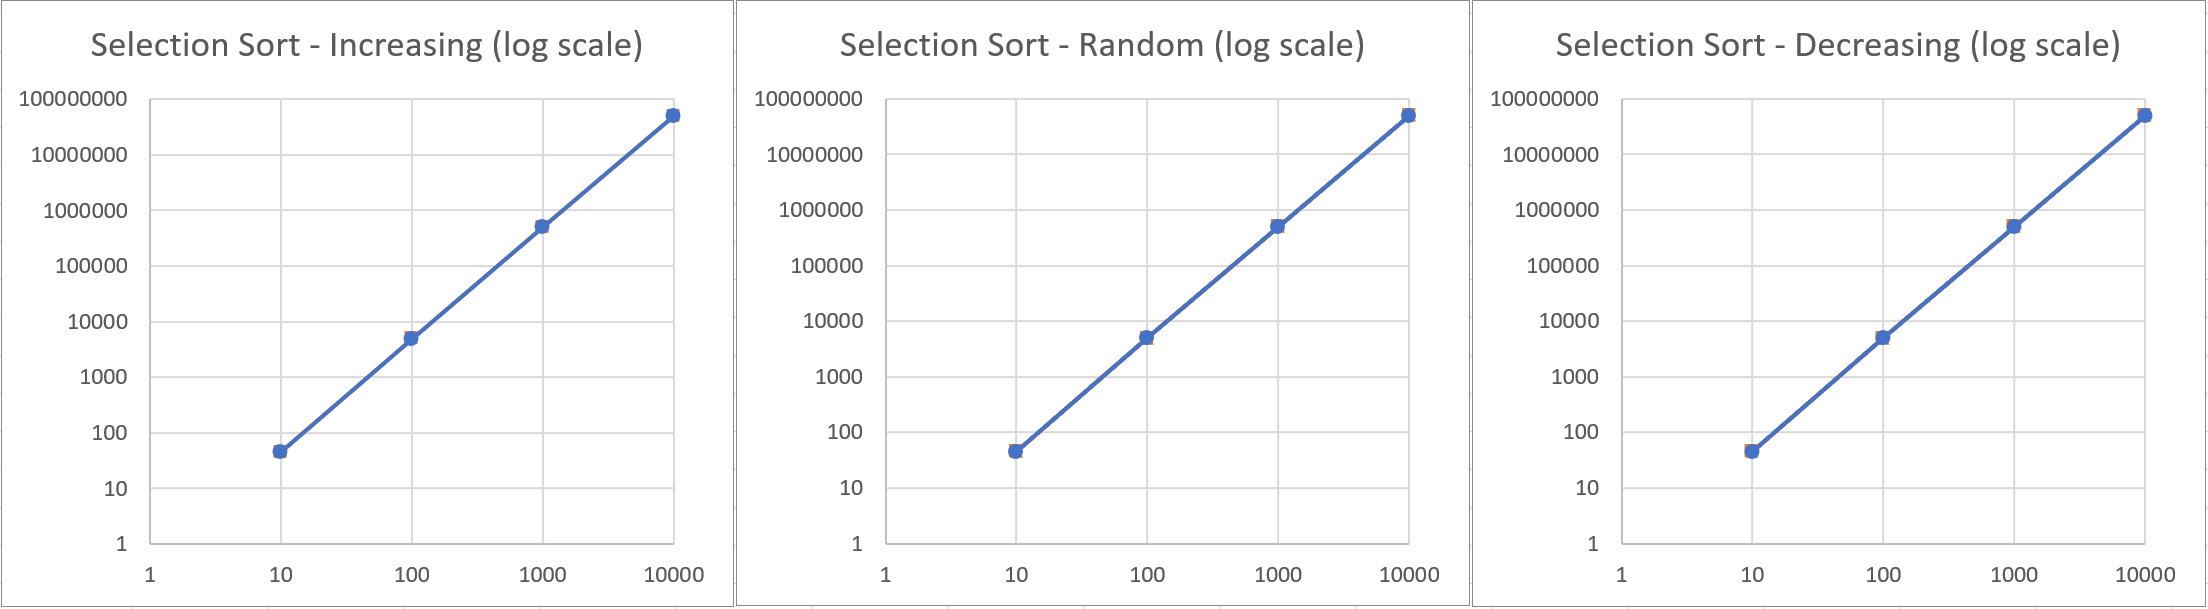
\includegraphics[width=\textwidth,height=\textheight,keepaspectratio]{SelectionSort.png}\ \\
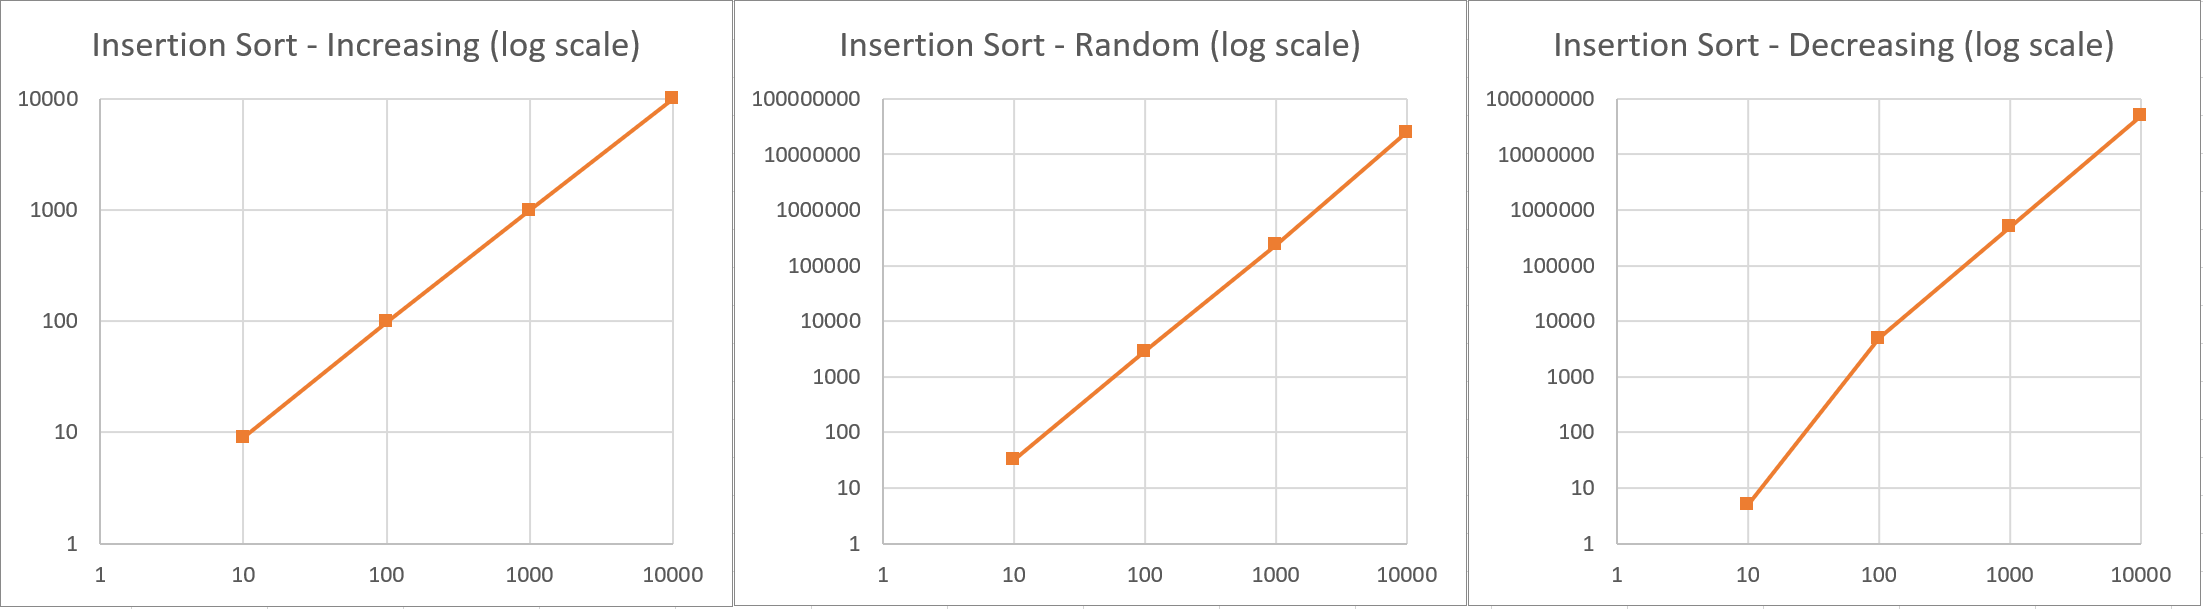
\includegraphics[width=\textwidth,height=\textheight,keepaspectratio]{InsertionSort.png}\ \\
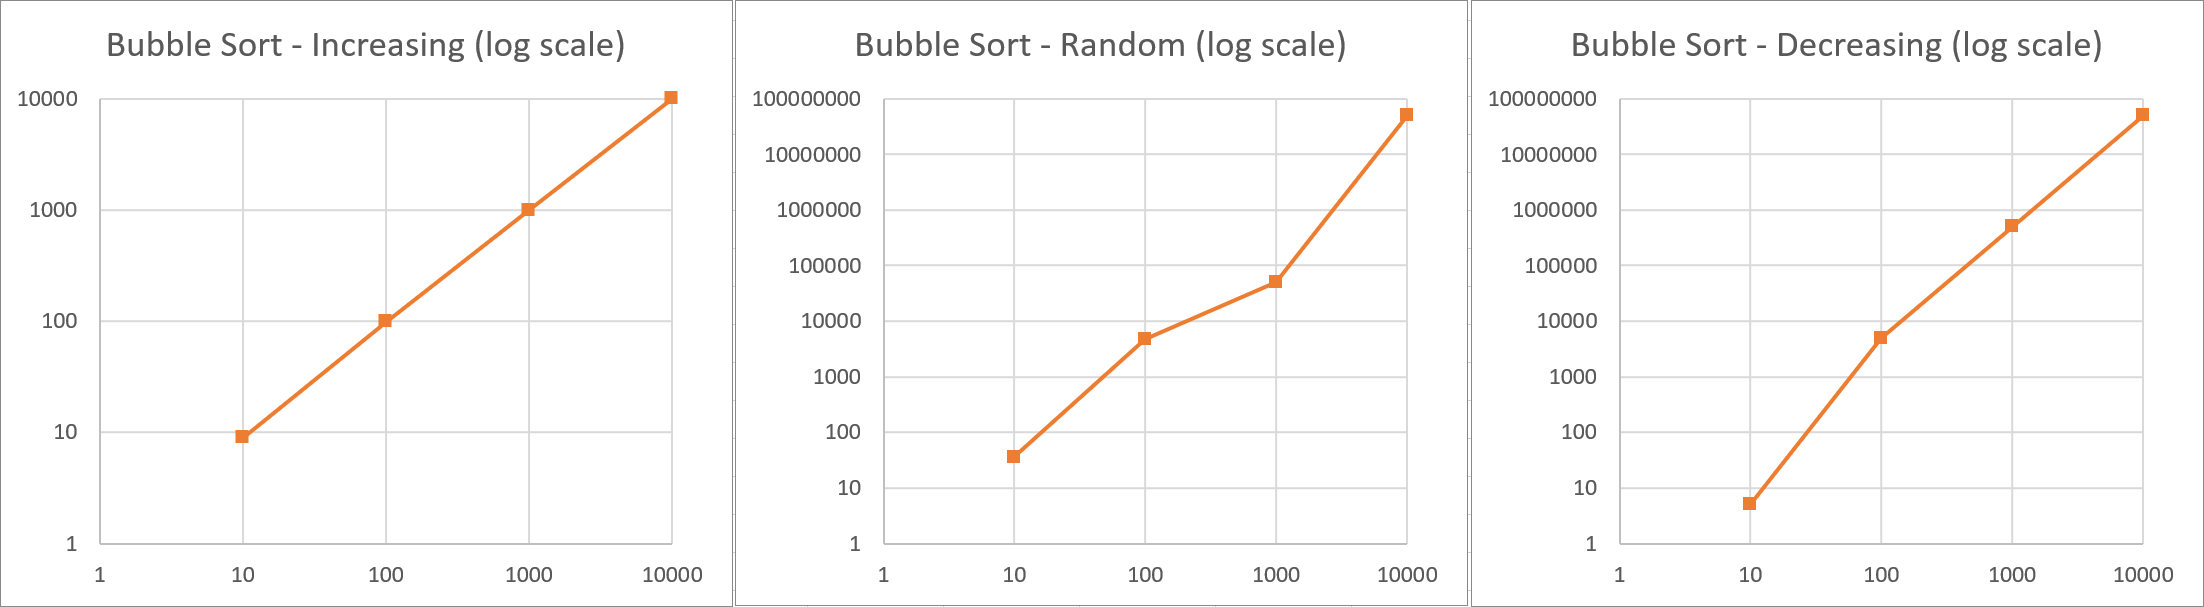
\includegraphics[width=\textwidth,height=\textheight,keepaspectratio]{BubbleSort.png}\ \\
\ \\
\item Testing \ \\
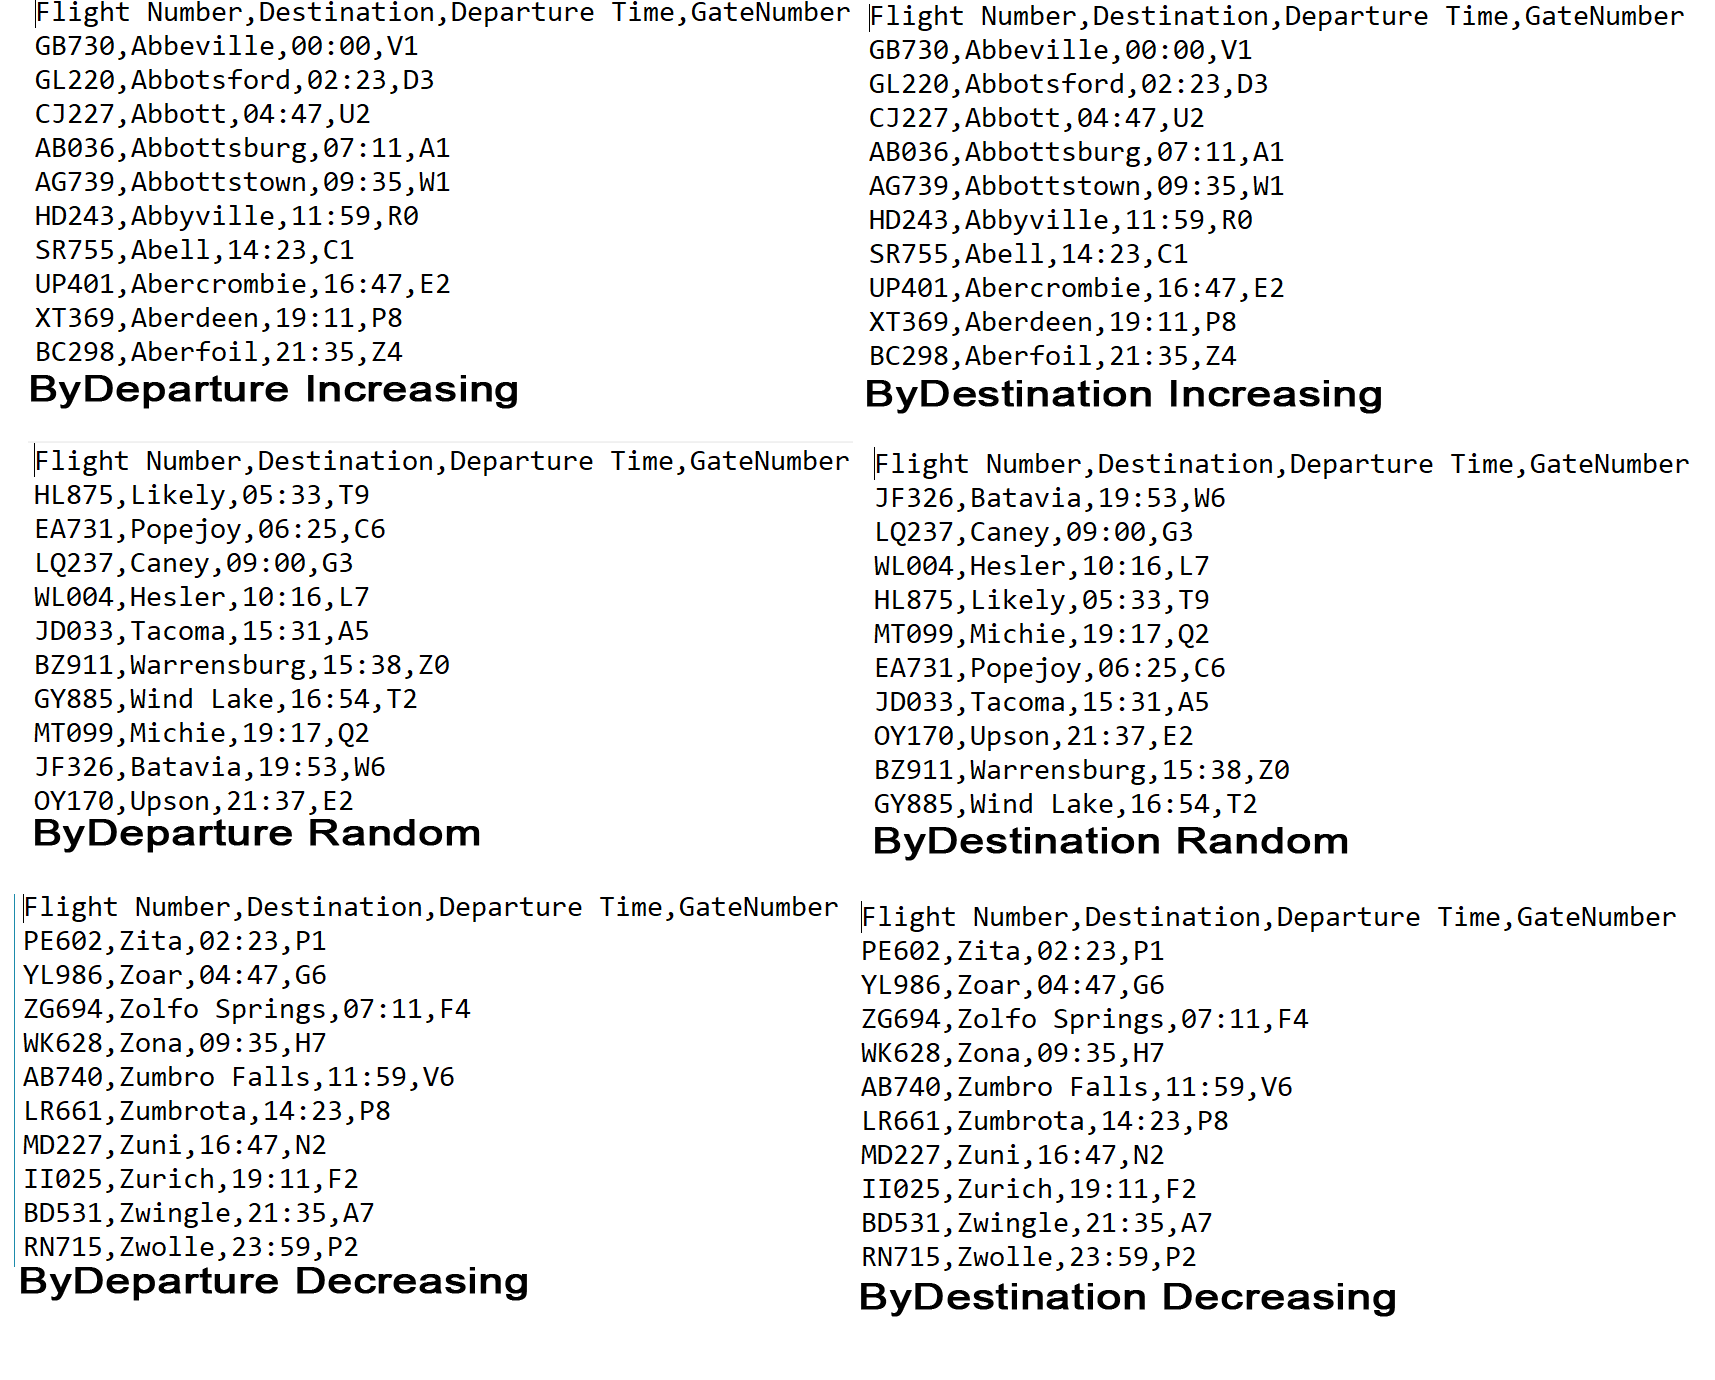
\includegraphics[width=\textwidth,height=\textheight,keepaspectratio]{TestTable.png}\ \\
\item \textbf{Discussion.} Comment on how the experimental results relate
to the theoretical analysis and explain any discrepancies you note.
Do your computational results match the theoretical analysis you learned
from class or the textbook? Justify your answer.\ \\

The experimental results fell closely in line with the theoretical analysis. Best, average, and worst cases corresponded with increasing, random, and decreasing data sets. For selection sort all three cases remained the same, which correlated to the theoretical analysis that stated the best, average, and worst cases would always be equal $O(n^2)$. Bubble and insertion also ran as expected. Both of these algorithms perform best when used on data sets that are already partially sorted. In both best cases tested where the values were already sorted, the algorithm was only required to make comparisons until it was determined that the values were already ordered $O(n)$. In worst cases, every item had to be compared to every item and was equivalent to $O(n^2)$.
\ \\
\ \\
\ \\
\ \\
\ \\
\item \textbf{Conclusions.} Give your observations and conclusion. For instance,
which sorting algorithm is more suitable for a specific input data?
What factors can affect your experimental result?\ \\
\ \\
Selection sort is a basic algorithm that would only be useful on very small inputs. Insertion sort and bubbles both have similar ideal situations. They work best on inputs that have already been somewhat sorted. A factor that could affect experimental results would be the order of the random values. Ideally, multiple sets of random values would need to be tested in order to find a proper average.  

\ \\ 
\ \\
\ \\
\end{enumerate}
\end{enumerate}
\noindent \begin{flushleft}
\textbf{\textcolor{black}{Turning In }}
\par\end{flushleft}
\begin{enumerate}
\item Use \texttt{\textcolor{black}{\small{}tar }}program to bundle all
your files in one file. 
\item Do not turn in the object files and/or executable file. 
\item Note: Late projects are penalized according to the weights provided
in the syllabus.
\item If your program does not compile on a Linux machine or if there are
run-time errors, you will get at most 50\% of the total number of
points.
\end{enumerate}

\end{document}
